\subsection{Mokymasis su mokytoju ir mokymasis be mokytojo}

Šiame skyriuje atsakysiu į klausimą kuo skiriasi mokymasis su
mokytoju (angl. supervised learning) nuo mokymosi be mokytojo (angl.
unsupervised learning). Mokymasis, duomenų klasifikavimo kontekste, reiškia modelių(pvz. klasifikatorių) kūrimo metodus (algoritmus), kurie naudoja
mokymosi duomenis\footnote{Mokymosi duomenys (angl. sample data)- duomenys,
kurie yra paruošti darbui programų, kurios kurs modelius (pvz.
klasifikatorius).}, kitaip tariant, tai mokymasis iš pavyzdžių.

\subsubsection{Mokymasis su mokytoju}

Mokymasis su mokytoju tai toks mokymasis, kai turime mokymosi duomenis, kuriems jau
yra priskirtas tam tikras teisingas atsakymas. Kitaip tariant, mes sprendžiame
uždavinį, kuriam atsakymą galime pasitikrinti. Mokymasis su mokytoju yra
skirstomas į dvi rūšis:
\begin{enumerate}
  \item Klasifikavimas (angl. classification) - pagal nepriklausomus
  kintamuosius bandome nuspÄ—ti kokybinius (kategorinius) priklausomus kintamuosius. 
  \item Regresija (angl. regression) - pagal nepriklausomus kintamuosius bandome
  nuspÄ—ti kiekybinius priklausomus kintamuosius.
\end{enumerate} 

%% JG: Pateik vizualų klasifikavimo pavyzdį iliustruojanti visus 3 etapus.
%% DJ: Vizualų, ta prasme su paveiksliukais ar ir tas pavyzdys su paštu
% pakankamai vaizdingas?

%% JG: Reikia kitaip struktūrizuoti šitą skyrių: 
% +Pradžioj pasakyk, kad yra klasifikavimas ir regresija ir po
%  sakinį kiekvienam.
% +Tada aptark klasifikavimą ir pateik pavyzdį. 
% +Tada pateik regresijos pavyzdį.
% +Tada parašyk, kad šiame darbe studijuojama klasifikavimo problema.

\paragraph{Klasifikavimo uždavinio pavyzdys}

Klasifikavimo tikslas - identifikuoti parametrus, kurie nusakytų grupę (klasę),
kuriai priklauso objektas. Klasifikavimo sąvoka gali būti naudojama tiek esamų
duomenų suvokimui, tiek naujų objektų charakteristikų prognozavimui.
Klasifikavimo uždavinių aktualumą galima parodyti tokiu pavyzdžiu.

\begin{figure}[htb]
\begin{center}
\leavevmode
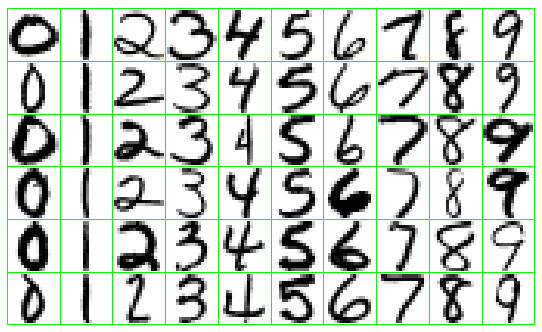
\includegraphics[width=0.5\textwidth]{images/ranka_rasyti_skaiciai.png}
\end{center}
\caption{Ranka rašytas tekstas, kurį reikia atpažinti.}
\label{fig:flash}
\end{figure}

Uždavinys: Pašto skyriuose laiškai siun�iami įvairiomis kryptimis pagal gavėjo
adresą ir (arba) pašto kodą. Norima automatizuoti laiškų rūšiavimą pagal
siuntimo kryptį. Tam, kad būtų galima laiškų rūšiavimą pagal kryptį
automatizuoti, mums reikia priemonės atpažinti ant voko užrašytą
pašto kodą.

Sprendimas: Šią problemą mums padėtų išspręsti skeneris ir programine įranga,
kuri sugebėtų ranka rašytus skaitmenis atpažinti ir konvertuoti į skaitmeninį
formatą. Tų skaitmenų atpažinimui ir konvertavimui į skaitmeninį formatą
mes naudosime klasifikavimo algoritmus, nes uždavinys pasižymi
visomis klasifikavimui būdingomis savybėmis: turime aibę duomenų (vaizdinė
informacija su ranka rašytais skaitmenimis), turime teisingus atsakymus (žmogus
pažiūrėjęs į ranka rašytą skaitmenį gali pasakyti programai, koks ten yra
skaitmuo), bei galimų sprendimai yra kategorinio tipo (dešimt skaitmenų nuo
0 iki 9).

Klasifikatorių kursime trimis etapais:
\begin{enumerate}
  \item diskriminavimo (atskirian�iųjų) kintamųjų parinkimas - nuskenuotų
  pašto kodų skaitmenų dažniausiai pasitaikan�ių, charakteringiausių linijų
  radimas,
  \item klasifikavimo taisyklių sudarymas - pagal tam tikrą charakteringiausių
  linijų grupę objektui priskiriama klasė,
  \item klasifikavimo kokybės įvertinimas - kokybei įvertinti naudojami įvairūs
  metodai, tokie kaip kryžminis patikrinimas (angl. cross-validation) ir
  įkel�ių metodas (angl. bootstrap).
\end{enumerate}

Įgyvendinę aukš�iau aprašyto uždavinio sprendimą, pašto skyriaus vadybininkai
galėtų atlaisvinti žmones nuo iš esmės mechaninio darbo - rūšiuoti laiškus.
Tokiu būdu būtų optimizuotas pašto skyrių efektyvumas.

\paragraph{RegresinÄ—s analizÄ—s payzdys}

Regresija prognozuojant naujų duomenų reikšmes naudojasi žinomais, jau turimais
duomenimis. Ji naudoja standartinius statistinius metodus, tokius kaip mažiausių
kvadratų metodas (angl. least squares). Regresinė analizė dažniausiai naudojama
įvertinti (ang. forecast) ateities duomenų vertes bei interpoliacijai -
funkcijos tikėtinos reikšmės tarp dviejų taškų įvertinimui.

Tipinio uždavinio, kuriam naudojama regresinė analizė pavyzdys: Aktuarinėje
(draudimo) matematikoje reikia turėti įver�ius, pasakan�ius kokia tikimybė, kad
žmogus vienokio ar kitokio amžiaus mirs. Tam yra naudojamos taip vadinamos 
mirtingumo lentelės. Jose duomenys aprašo kiek ir kokio amžiaus žmonių
kažkuriais metais mirė, pvz. 2010 metais Lietuvoje mirė 1000 20 metų amžiaus 
žmonių. Detalesni duomenys nėra naudojami, nes per daug sudėtinga juos apdoroti.
Kadangi aktuarai nori apskai�iuoti draudimo kainą, jiems reikia įvertinti
riziką, kada žmogus mirs, tai jie naudodamiesi regresinės analizės metodais 
paskai�iuoja tikėtiniausią reikšmę, kad pvz. yra 3\% tikimybė, kad žmogus  mirs
dvidešimtaisiais savo gyvenimo metais. Kitais žodžiais tariant, iš turimų
duomenų mes sukursime tolydžią funkcija, kuri mums pasakys reikšmes taškuose,
kurių mes neturime.

\paragraph{Klasifikavimas ir regresija}

Abiejų mokymosi su mokytoju rūšių tikslas yra pagal mokymosi duomenis sukurti
modelį, kuriuo remiantis būtų galima identifikuoti naujų objektų
savybes.\cite{markhall99} Å iame darbe negrinÄ—sime klasifikavimo problemÄ….

\subsubsection{Mokymasis be mokytojo}

Mokymasis be mokytojo tai toks mokymasis, kai turime mokymosi duomenis, kuriems
nėra priskirtas teisingas atsakymas. Kitaip tariant, mes sprendžiame
uždavinį, kuriam atsakymo galime pasitikrinti. Mokymosi be mokytojo principas - 
maksimizuoti objektų, esan�ių vienoje grupėje, tarpusavio panašumą ir 
minimizuoti tarpgrupinį objektų panašumą.

Mokymosi su mokytoju metu galima išmatuoti gauto modelio tikslumą įvairiais metodais, pvz.
kryžminiu patikrinimu. Mokymesi be mokytojo mes tokių tiesioginio patikrinimo
procedūrų neturime. Todėl yra sunkiau išsiaiškinti patikimumą išvadų, gautų pagal
daugumos mokymosi be mokytojo algoritmų darbo rezultatus. 

Yra mažiausiai penkios pagrindinės priežastys, kodėl mums gali būti įdomūs
mokymosi be mokytojo algoritmai:

\begin{enumerate}
	\item Turime labai daug nesužymėtų (angl. unlabelled) duomenų, o jų
	sužymėjimas rankomis būtų labai brangus. 
	\item Norime apsimokyti su dideliu kiekiu sąlyginai ,,pigių`` duomenų tam,
	kad paskui galÄ—tume	pasitelkti mokymosi su mokytoju algoritmus, ir tada
	detaliau ištirti duomenis.
	\item Duomenų struktūros šablonas yra nuolat kintantis, ir jei tą kitimą
	galėtume sekti mokymosi be mokytojo režimu, tai būtų galima padidinti 
	mūsų programos našumą.
	\item Galima panaudoti mokymosi be mokytojo algoritmus, kad surastume
	duomenų savybes, kurias vėliau panaudosime duomenų kategorizavimui.
	\item Pradinėje duomenų analizės stadijoje pasinaudoję mokymosi be mokytojo
	metodais galime geriau pažinti turimus duomenis.
\end{enumerate}

Mokymosi be mokytojo algoritmų pagrindinis privalumas – gebėjimas atpažinti grupavimo
struktūrą be jokios išankstinės informacijos.

%% JG: neprižiūrimų mokymosi metodų yra visokių: association rule mining,
% clustering, ir t.t. Zr ESL knygos 14 skyrių.
%% DJ: Nurašinėjau nuo Duda knygos tą vietą, kur mokymas be mokytojo ir 
% klasterizavimas yra sinonimai.

%% Kartais šiokia tokia informacija žinoma. Pvz., klasterių kiekis nurodomas
% k-means algoritme. Arba galima daryti prielaidas apie klasterių struktūrą:
% k-means ieško apvalių klasterių. Esminis dalykas yra tas, kad teisingas
% atsakymas nėra žinomas.

%% JG: algoritmas turi atrasti grupes duomenyse, jos nėra iš anksto žinomos.

\subsubsection{Mokymosi su mokytoju ir mokymosi be mokytojo skirtumai}

Pagrindiniai skirtumai tarp mokymosi su mokytoju ir mokymosi be mokytojo yra:
\begin{itemize}
	\item mokymosi duomenys - mokymosi su mokytoju algoritmų įeities duomenyse
	yra	išreikštinai pasakyta, kokio rezultato mes laukiame, o mokymosi be
	mokytojo įeities duomenyse tokios papildomos informacijos nėra.
	\item  naudojimo tikslai - mokymasis su mokytoju siekia iš pavyzdžių
	išmokti vertinti naujus duomenis, o mokymasis be mokytojo siekia atrasti
	vidinę duomenų struktūrą.
\end{itemize}

Aptarkime pavyzdį: nuotraukų apdorojimas.

Mokymosi su mokytoju programai kaip įeities duomenis paduotume keletą 
nuotraukų su žymėmis pasakan�iomis, ar nuotraukoje yra žmogaus veidas ar jo ten
nėra, kitaip tariant, duotume keletą pavyzdžių su teisingais atsakymais.
Programa peržvelgs visas nuotraukas ir susikurs klasifikatorių (modelį), kuris
kažkokiu tikslumu galės atskirti nuotraukas su žmogaus veidu. Tokiu būdu mūsų
mokymosi programa ,,išmoks`` nuotraukose atpažinti veidus.

Mokymosi be mokytojo programai kaip įeities duomenis paduotume keletą
nuotraukų be jokių papildomų žymių. Žinoma, mūsų programa pati nesugebės
,,išrasti``, kas yra žmogaus veidas, ta�iau ji tikriausiai sugrupuos nuotraukas
su žmonių veidais ir tarkim peizažais į skirtingas grupes. Kitaip tariant,
nuotraukų su žmonių veidais vidinė struktūra mūsų mokymosi be mokytojo programai
bus nepanaši į nuotraukų su peizažais vidinę struktūrą, todėl ji į vieną grupę
sudės nuotraukas, kurios jai atrodo tarpusavyje panašiausios: vienoje
grupėje nuotraukos su žmonių veidais, o kitoje su gamtos peizažais.

Abu mokymo procesai yra panašūs savo esme (siekia išgauti žinias apie turimus
duomenis), bet jų panaudojimas skiriasi iš esmės (mokymo su mokytoju atveju mes
kuriame modelį apibūdinantį kaip buvo sukurti mokymo duomenys, kad galėtume
spėti naujų objektų savybes, o mokymo be mokytojo atveju siekiame susipažinti
su vidine mokymo duomenų struktūra, kai nėra kaip pamatuoti ar geri ar blogi
klasteriai buvo rasti).

%% JG: aš nesutinku, kad abiem procesais siekiama tų pa�ių tikslų. Vienu atveju 
% siekiama išmokti iš pavyzdžių. Kitu atveju siekiama atrasti nežinomas
% struktūras turimuose duomenyse. Procesai yra panašūs savo esme, bet jų 
% panaudojimas skiriasi iš esmės.

%% JG: iš vikipedijos: In machine learning, unsupervised learning refers to the 
% problem of trying to find hidden structure in unlabeled data. Since the
% examples given to the learner are unlabeled, there is no error or reward
% signal to evaluate a potential solution. This distinguishes unsupervised 
% learning from supervised learning and reinforcement learning.

%% JG: visą šitą skyrių reikia pateikti koncentruotai. Esminiai teiginiai ir grafiniai pavyzdžiai. 

%% DJ: Turiu pripažint, kad šitam pavyzdyje prigrybavau stipriai. Nurašinėjau
% pavyzdį kur prastai paaiškino skirtumą, bet užtat man pavyzdys patiko. Dabar
% labiau į temą surašyta.
